Latex ermöglicht es aus Textdateien formatierte PDF Dokumente zu erstellen. Ähnlich der Buchfunktion im Wikipedia. Außerdem können Ausgaben von Programmen ansprechend formatiert ausgegeben werden.\\
Durch das Einbinden von externen Dateien können Textbausteine, Layouts oder Bilder zentral abgelegt werden. Beispielsweise können dadurch Layout, Adresse oder Logo eines Vereins einfach in allen Dokumenten gleichzeitig verändert werden. Die Dokumente müssen nur neu compiliert werden.\\
Ich verwende als Editor den Texmaker und als Latex Distribution Miktex. Sollte es dazu Fragen geben einfach mal an mich wenden.\\

\begin{minipage}[t]{\textwidth}
  \centering
  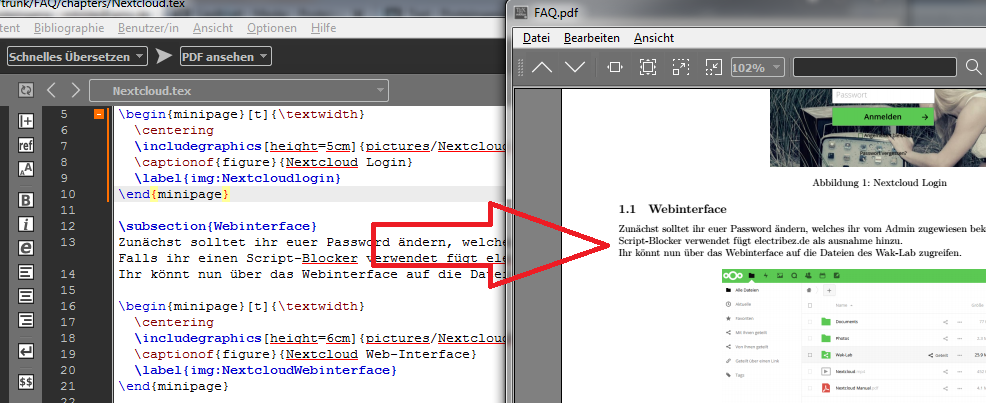
\includegraphics[width=\textwidth]{pictures/Texmaker.png}
  \captionof{figure}{Texmaker}
  \label{img:Texmaker}
\end{minipage}



